%Modelo de relatório de Transformações Bioquímicas em Latex (2009/3)
%Escrito por Amadeus Folego da Silva
\documentclass[a4paper, oneside]{report}                        %classe relatório, papel A4, formato de uma página
\usepackage[top=3cm, bottom=2cm, left=3cm, right=2cm]{geometry} %margens da folha
\usepackage[utf8]{inputenc}                                     %|
\usepackage[brazil]{babel}                                      %|adaptações para português brasileiro
%\usepackage{pslatex}                                           %fonte Times New Roman
\usepackage[alf]{abntex2cite}                                      %pacote de citações formato alfanumérico da abnt
\usepackage{indentfirst}                                        %começa parágrafo sempre
\usepackage{fancyhdr}                                           %pacote para editar layout da pagina
\usepackage{graphicx}                                           %pacote para colocar gráficos
\usepackage{amsmath}                                            %pacote para notações matemáticas da ams
\usepackage{url}                                                %pacote para colocar endereço online
\usepackage{listing}
\cfoot{}                                                        %nada no rodapé central
\rfoot{\thepage}                                                %número da página no rodapé à direita
\setlength{\headheight}{15pt}
\pagestyle{fancyplain}                                          %utiliza layout estabelecido

%\setlength{\parindent}{2.5cm}                                   %parágrafo com recuo de 2.5cm
\fontsize{12pt}{1.5cm}                                          %fonte tamanho 12, entrelinhas de 1.5cm

\title{\Huge{Universidade do Estado de Santa Catarina}\\[1.5cm]\huge{Projeto de Arquivos}\\[3cm]\large{\textbf{ORDENAÇÃO EXTERNA PELO METÓDO - SELEÇÃO POR SUBSTITUIÇÃO E A INTERCALAÇÃO DE N CAMINHOS}}\\[4cm]}  %título editado

\author{\hfill \textbf{Grupo}\smallskip\\\hfill Alexandre Maros\\\hfill Mateus Boiani\\\hfill \medskip\\\hfill \textbf{Prof. Responsável}\smallskip\\\hfill Wesley Bezerra} %autores editado

\date{\vfill\today}                                           %data

\begin{document}                                                %inicia documento

\maketitle                                                      %faz capa
\tableofcontents                                                %faz sumário

\renewcommand{\abstractname}{Resumo}                            %coloca nome de abstract para resumo
%\begin{abstract}                                                %inicia abstract
%Aqui você coloca o resumo do seu trabalho.                                                  %coloca resumo
%\end{abstract}                                                  %finaliza abstract

\chapter*{Introdução}                                           %inicia capítulo sem numeração
\addcontentsline{toc}{chapter}{Introdução}                      %como não numeramos os capítulos, precisamos fazer isso pra colocar a introdução no sumário
Muitas vezes nos deparamos com quantidades finitas de dados desorganizadas em nossas estruturas, e precisamos organizá-las. Por sorte, quando todos os dados de nossas estruturas cabem na memória fica mais fácil realizar está tarefa. Conhecemos vários algoritmos clássicos para isso, Quick Sort, Bubble Sort, Merge Sort, entre outros.\par
Mas quando a quantidade de dados que estamos manipulando e precisamos ordenar não cabe na nossa memória, como fazemos para alcançar nosso objetivo? Adicionamos mais memória no computador para executar esta tarefa parece ser uma resposta bastante trivial, não é? A verdade é que esse problema é mais antigo do que imaginamos, e muitos cientistas da computação criaram soluções que resolvem esse problema.\par
Vamos aqui explorar apenas uma das soluções existentes, ver quanto tempo o algoritmo leva para organizar essas informações e analisar esses resultados.


\chapter*{Objetivos}
\addcontentsline{toc}{chapter}{Objetivo}
O objetivo desse trabalho é apresentar o algoritmo de ordenação externa utilizando o método da seleção por substituição.\par
Apresentar de forma didática e intuitiva o funcionamento do algoritmo já citado demonstrando como é possível organizar um arquivo de dados que não podem ser carregados simultaneamente na memória para que seja feita a ordenação dos mesmos, também demonstraremos o tempo que este mesmo algoritmo leva em média para ordenar um arquivo de tamanho definido a seguir.\par
\chapter*{Problemática}
\addcontentsline{toc}{chapter}{Problemática}
\setcounter{chapter}{+1}

Ao introduzir uma linguagem de programação é comum nos ensinarem a organizar conjuntos de dados (um conjunto de números inteiros, float, double, etc;). Esses conjuntos de dados podem ser mantidos em uma estrutura de dados que conhecemos como vetores e/ou matrizes, esses vetores e matrizes são blocos de memórias sequências que são responsáveis por facilitar a manipulação e acesso a informação que desejamos manipular.\par
Quando precisamos organizar esse conjunto de dados em ordem crescente, decrescente ou seguindo algum padrão específico é comum utilizarmos algoritmos de organização como o bubble sort, por exemplo. Quando trabalhos com um conjunto de dados que cabe na memória e queremos organiza-lo denominamos Classificação Interna.\par
Os dados que não são suportados na memória e que queremos organizar chamamos de Classificação Externa. E para organizar e manipular esses dados foram criados diversos algoritmos. Veremos a seguir o método de substituição por seleção e a intercalção de n caminhos.

\section{Classificação Externa}

Os dados que queremos organizar estão salvos em um arquivo, a classificação externa que utilizamos para organizar estes dados pode utilizar esse arquivo original ou um arquivo auxiliar, e consiste de dois passos.\par
\textbf{Classificação:} São geradas partições(arquivos) de n registros ordenados. \par
\textbf{Intercalação:} É a transformação das partições criadas na classificação em uma única partição ordenada com todos os registros originais.\par
Tanto a Classificação quanto a Intercalação podem ser feitas por métodos variados métodos, aqui abordaremos a classificação utilizando seleção por substituição, e a intercalação de n caminhos.
\newpage
\subsection{Seleção por Substituição}

A seleção por substituição consiste basicamente da leitura do máximo de registros do arquivo original para memória, (1) selecionar o menor registro, gravar na partição de saída. Após gravar na partição de saída substituir o registro gravado pelo próximo registro do arquivo original, (2) selecionar o menor registro novamente, se o menor registro for menor que o último registro escrito no arquivo de saída então congelar este registro e ignorar no restante do processamento. Enquanto existirem registros não congelados executar a etapa (2) sucessivamente, caso contrário, fecha a partição de saída atual, descongela os registros congelados na memória, abrir nova partição de saída e executar a partir da primeira etapa novamente. 



\begin{figure}[h]
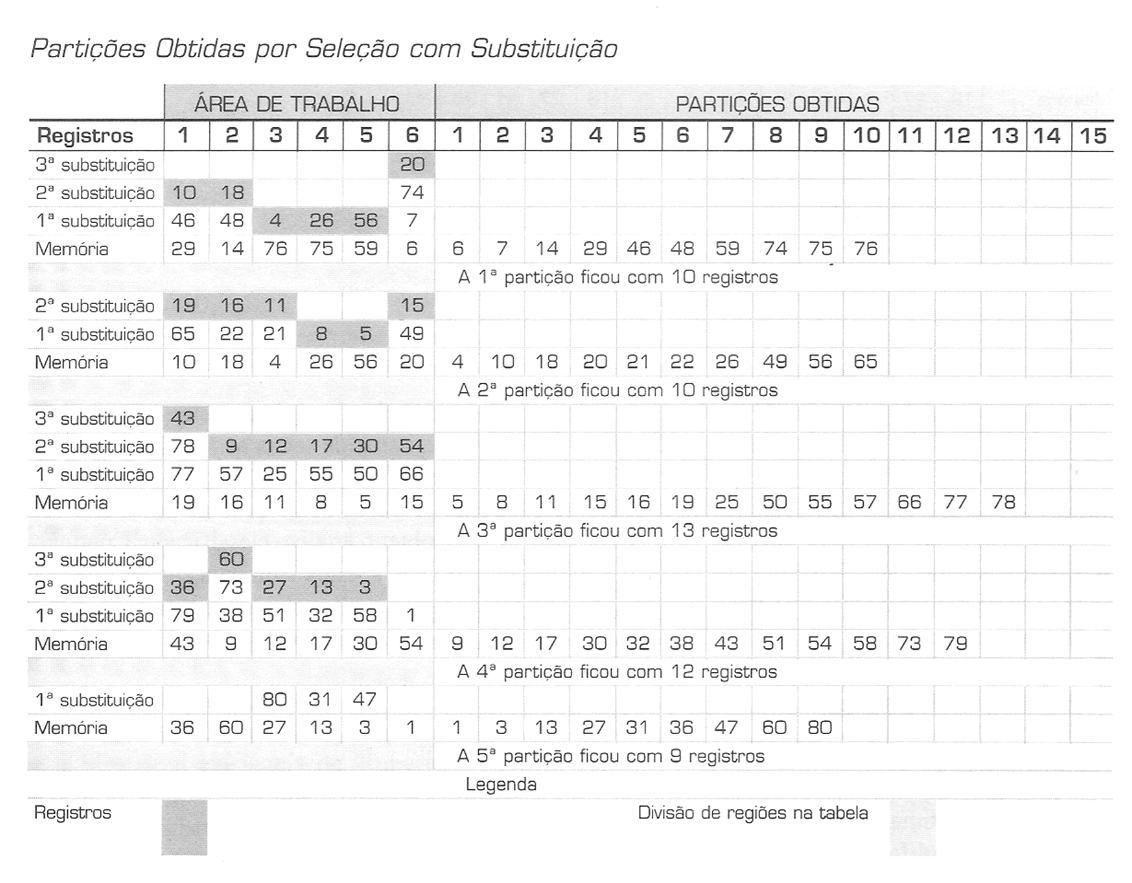
\includegraphics[width=.7\paperwidth]{selecao_com_substituicao}
\caption[align = center]{Seleção por Substituição} 
%FERRAZ, Inhaúma Neves. Programação com arquivos / Inahúma Neves Ferraz. - Barueri, SP : Manoele, 2003
\label{fig:selecao_com_substituicao}
\begin{center}
Fonte: FERRAZ, Inhaúma Neves - Programação com arquivos pg. 69
\end{center}
\end{figure}
Conforme a imagem acima, podemos observar o comportamento do método de seleção por substituição. Os registros que contém fundo escurecido são os registros que ficaram congelados e que serão utilizados no arquivo subsequente. Podemos observar que nesta etapa pode ocorrer a criação de inúmeros arquivos, e o processo só irá terminar quando não tivermos mais nenhum registro na memória e nenhum registro congelado. 
\newpage

\subsection{Balanceamento de N Caminhos}

Como vimos anteriormente a intercalação é a transformação das partições criadas na classificação em uma única partição ordenada. Para isso vamos utilizar o método de balanceamento de N caminhos.\par
Esse método consiste na união dos arquivos gerados na classificação. São N etapas unindo arquivos em duplas, ou seja, cada dois arquivos gerados na classificação um novo arquivo é gerado a partir da união. Para isso é feito a leitura registro a registro e comparando ambos. Como os arquivos estão ordenados já, então é só comparar e ir salvando um por um no novo arquivo. Ao final das N etapas teremos um arquivo final com todos os registros ordenados. Você deve estar se perguntando, mas se eu tiver um número ímpar de arquivos gerados na classificação? Isso realmente pode acontecer, para resolver isso, costumamos pegar o arquivo que sobrou na enésima etapa e unir com o primeiro arquivo gerado da etapa seguinte.

\begin{figure}[h]
\includegraphics[width=.7\paperwidth]{balanceamentoNcaminhos}
\caption{Balanceamento de N Caminhos}
\label{fig:balanceamentoNcaminhos}
\end{figure}

A ilustração acima retrata exatamente o que acontece ao intercalação, buscamos os N arquivos criados na classifição e realizamos a união em pares. Como a classificação neste caso gerou uma quantidade ímpar de arquivos, pegamos esse arquivo para utilização inicial na iteração seguinte. Isso é feito para evitar que um arquivo de tamanho muito pequeno seja mantido até o final das iterações. Neste caso garantimos que 2 arquivos de tamanhos semelhantes cheguem para ultima iteração. 

\chapter*{Experimento}
\addcontentsline{toc}{chapter}{Experimento}
\setcounter{chapter}{+2}

\section{Informações Técnicas}
Rodamos os algoritmos anteriormente apresentados, e vamos mostrar os resultados obtidos. Sobre a máquina:
\newline

\textbf{Disco Rígido:} Seagate ST1000DM003-1ER162 7200rpm;
\par
\textbf{Processador:} Intel Core i7-4790K CPU @ 4.00Ghz;
\par
\textbf{Memória:} 8,00 GB 1600Mhz;
\par
\textbf{Sistema Operacional:} Windows 8.1 Pro;
\newline

Sobre o arquivo a ser ordenado e o algoritmo:
\par
\textbf{Estrutura utilizada:} Estrutura denominada medição, contendo índice, temperatura variando de 0 a 50 graus, dia, mês, ano, sendo todos os campos do tipo long long (8 bytes);
\par
\textbf{Tamanho de cada medição:} 40 bytes; 
\par
 
\textbf{Quantidade de medições:} 322.122,547;
\par

\textbf{Tamanho total do arquivo:} 12,0 GB = 12.884.901.888 bytes;
\par
\textbf{Linguagem em que o algoritmo foi escrito:} Linguagem C;
\par
\textbf{Forma de ordenação:} Crescente, ordenando a temperatura;
\newpage

\section{Resultados}

\textbf{Tempo para gerar o arquivo inicial em média:} 98 segundos;
\par

\begin{figure}[h]
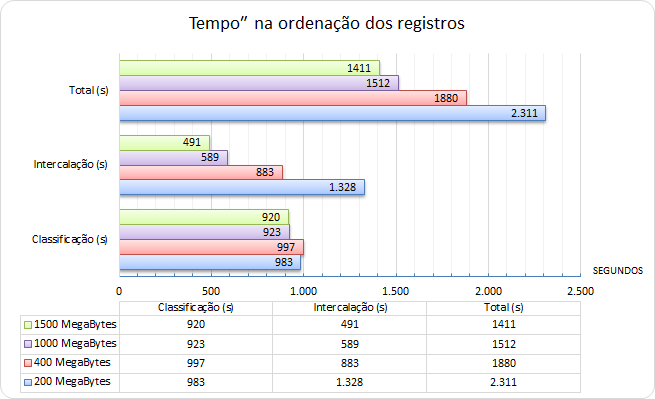
\includegraphics[width=.7\paperwidth]{tempoOrdenacaoRegistros}
\caption{Tempo para Ordenar 12GB dividindo em blocos de N MegaBytes carregados na memória.}
\label{fig:tempoOrdenacaoRegistros}
\end{figure}
Obs.: Esses valores são aproximações.


\subsection{Análise dos Resultados}
\par
No gráfico acima, tem-se os resultados dos experimentos realizados em cima do algorítmo de ordenação. Temos três grandes sessões, uma mostrando o tempo total do algorítmo, uma mostrando somente o tempo necessário para a etapa da intercalação e por fim, a ultima sessão mostra o tempo de classificação. Os testes foram realizados alterando o tamanho do bloco carregado na memória (1500, 1000, 400 e 200 MegaBytes) em um deteminado instante e o tempo foi medido em segundos.
\par
\textbf{Tempo de intercalação:} Aqui nota-se uma discrepância nos tempos de cada bloco. O maior bloco, 1500 MB, realizou a operação de intercalação em aproximadamente 8 minutos, ja quando carregamos apenas um bloco de 200 MB, seu tempo subiu para 22 minutos. Isso ocorre devido ao fato de que, quando um bloco maior é carregado na memória, este gera menos arquivos na etapa de classificação, logo, o Sistema Operacional realiza menos operações para abrir e fechar arquivos, ocasionando num tempo total muito menor.
\par
\textbf{Tempo de classificação:} Na classificação, o tempo se manteve estável e não se diferenciou muito com o aumento dos blocos. Embora ele necessite criar menos arquivos quando há um bloco maior na memória, ainda assim, ele trabalha com menos blocos que a etapa de intercalação.
\par
Para se ter um desempenho maior no algorítmo, um maior bloco deve ser utilizado em sua execução visando a criação da menor quantidade de arquivos possíveis. É necessário ter um cuidado especial na seleção do bloco, pois precisa-se levar em consideração a quantidade máxima de memória que o sistema operaciona consegue ceder sem que ele mesmo seja prejudicado devido a swap e outros fatores.
\chapter*{Conclusão}
\addcontentsline{toc}{chapter}{Conclusão}
Em geral, podemos ver que é possível ordenar arquivos grandes o suficiente tal que a memória não consiga comportar. Para isso dispomos de vários métodos de classificação e intercalação, aqui utilizamos a classificação pelo método de seleção por substituição e o balanceamento de n caminhos.
\par
O tempo total do ordenamento se dá por diversos fatores, sendo eles tempo de escrita e leitura do disco, tempo de processamento das informações na memória, criação de novos arquivos, abertura de arquivo, alocação de informação, são alguns exemplos. Escrever no disco rígido leva mais tempo do que indexar e trabalhar com registros na memória, vimos que com um arquivo muito grande, não é possivel carregar todos os registros na memória, ordenar, e salvar novamente, para que essa tarefa seja possível é necessário muitas operações de escrita e leitura do disco.
\par
Abordamos aqui um dos métodos clássicos para ordenar uma quantidade enorme de dados, atualmente temos uma infinidade de outros métodos para realizar este tipo de tarefa. 



%\bibliographystyle{abnt-alf}                                    %define estilo de bibliografia como abnt
%\bibliography{Bibliografia}                                     %coloca bibliografia

\end{document}                                                  %finaliza documento
